\section{把局部规律写成微分方程}
\subsection{未知量是一个函数}
牛顿定律 $m\ddot x=F$、电流关系 $I=\dot Q$、静水压关系 $\dd p/\dd z=-\rho g$，都只涉及某时刻或某位置附近的局部变化。当未知量是整个运动或分布函数时，这些规律就成为微分方程。解方程的任务是找到一个函数，使它在规定区间内处处满足局部规律，并符合初始或边界条件。

一阶方程通常需要一个初始条件，例如位置函数的速度规律配上 $x(0)=x_0$；二阶运动方程通常还需要 $v(0)=v_0$。由方程给出的函数族，不代入条件便不能确定具体运动。判断答案时应同时检查方程、初值与适用区间，而不只是看最终表达式是否熟悉。

物理建模应先明确研究对象和变量。若速度给成位置函数，选位置作为积分变量往往比先求时间函数更直接；若加速度只随速度变化，可以先解速度的一阶方程；若研究微小偏离平衡的行为，则先选偏移量，再把恢复作用展开到一阶。

\fig{c4k-initial}{相同方程的解由初始状态进一步确定}{\begin{tikzpicture}[x=1cm,y=.8cm]
\draw[axis](0,0)--(4.7,0)node[right]{$t/\tau$};\draw[axis](0,0)--(0,3.7)node[above]{$y$};
\foreach \a/\col in {1/black,2/blue,3/red}{\draw[\col,domain=0:4.2,samples=40]plot(\x,{\a*exp(-\x)});}
\fill(0,1)circle(1.4pt);\fill[blue](0,2)circle(1.4pt);\fill[red](0,3)circle(1.4pt);
\node[left]at(0,1){$C_1$};\node[left]at(0,2){$C_2$};\node[left]at(0,3){$C_3$};
\node at(3,2.3){$y=C\e^{-t/\tau}$};
\end{tikzpicture}}
图 \ref{c4k-initial} 的三条曲线都满足 $\dot y=-y/\tau$，却对应三个不同的初值。局部规律只规定“在当前状态怎样变化”，初始条件才指定从哪一点开始。对解作检验时，可先求导代回方程，再令起始时刻为零代入初值；两步都成立后，还要检查解是否一直留在模型允许的范围内。

初始条件与边界条件也不同。运动题通常给同一时刻的位置和速度；静态分布可能给两个不同位置处的条件。二阶方程形式相同，并不意味着条件可以任意搭配，尤其在分段介质和接触边界处，还应把函数或通量的连续条件与模型一同写出。

\subsection{可分离变量与平衡解}
若 $\dot y=f(t)g(y)$，在 $g(y)\ne0$ 的区间内可写成
\[
 \frac{\dd y}{g(y)}=f(t)\dd t,\qquad
 \int_{y_0}^{y(t)}\frac{\dd u}{g(u)}
 =\int_0^t f(s)\dd s.
\]
上下限已包含初值，因此不必再引入一个独立的不定积分常数。分离前必须检查 $g(y)=0$ 的解：例如 $\dot y=-\lambda y$ 除以 $y$ 后会暂时排除恒零解，但恒零解本来合法。

式中的微分形式建立在链式法则上，不是将任意导数符号当成普通分数随意约去。遇到不单调运动，应按区间求解；积分中出现对数时，还要根据初值确定符号与允许区间。

以 $\dot y=a y(1-y/K)$、$a,K>0$ 为例，若先除以 $y(1-y/K)$，会把 $y=0$ 与 $y=K$ 两个常值解排除在积分步骤之外。它们却直接满足方程，应先保留。对其余解，也无需立即算出显式函数就能判断变化方向：当 $0<y<K$ 时右侧为正，$y$ 增长；当 $y>K$ 时右侧为负，$y$ 减小。
\fig{c4k-equilibrium}{方程右侧的符号给出允许状态的变化方向}{\begin{tikzpicture}
\draw[axis](-.3,0)--(5.1,0)node[right]{$y$};
\fill(0,0)circle(2pt)node[below]{$0$};\fill(3,0)circle(2pt)node[below]{$K$};
\draw[flow,blue](.5,.1)--(1.5,.1);\draw[flow,blue](1.9,.1)--(2.7,.1);
\draw[flow,red](4.6,.1)--(3.4,.1);
\node[above]at(1.5,.25){$\dot y>0$};\node[above]at(4,.25){$\dot y<0$};
\end{tikzpicture}}
图 \ref{c4k-equilibrium} 中箭头指向 $K$，说明这个平衡状态能吸引邻近的正初值，而零状态对正向小扰动不稳定。求积分前先画这种方向关系，可以检查求得的指数、对数和分支是否符合实际变化。若模型右侧足够光滑，不同初值的解不能在同一时刻相交后又任意分开；达到平衡值的方式也受方程约束。

\subsection{量纲与时间尺度}
对方程 $\dot y=-y/\tau$，先取 $y_0\ne0$，在与初值同号的区间分离变量：
\[
 \int_{y_0}^{y(t)}\frac{\dd u}{u}
 =-\frac1\tau\int_0^t\dd s,
 \qquad [\ln|u|]_{y_0}^{y(t)}=-\frac t\tau.
\]
于是 $\ln|y/y_0|=-t/\tau$；由同号性取 $y/y_0>0$，得到 $y=y_0\e^{-t/\tau}$。求导检验为 $\dot y=y_0\e^{-t/\tau}(-1/\tau)=-y/\tau$，且 $y(0)=y_0$；$y_0=0$另有恒零解。指数必须无量纲，所以 $\tau$ 有时间单位；它表示初始量衰减到 $1/\e$ 所需时间。线性阻力的 $\tau=m/k$、RC 电路的 $\tau=RC$ 都出于这一结构。增长过程只改变指数的符号，但长期指数增长常受资源或其他效应限制，不能无限外推简单模型。

把时间改写为 $s=t/\tau$，原方程成为 $\dd y/\dd s=-y$；再令 $Y=y/y_0$，便得到 $\dd Y/\dd s=-Y$、$Y(0)=1$。不同质量的阻力运动与不同元件的电路，在各自时间尺度下具有同一条无量纲衰减曲线。图 \ref{c4k-initial} 中初值改变只作纵向缩放，时间尺度改变则作横向伸缩。

时间常数不是“到零所需时间”。在一个 $\tau$ 后剩下 $1/\e$，两个 $\tau$ 后剩下 $1/\e^2$，精确零值在理想指数模型中只于无限时间达到。若实验要求剩余比例小于 $\epsilon$，所需时间满足 $t>\tau\ln(1/\epsilon)$。半衰期则为 $\tau\ln2$，它与时间常数描述同一过程的不同计量方式。

\subsection{平衡值能否在有限时间到达}
方向关系能说明解趋向哪个平衡值，却不能单独给出到达时间。设衰减规律为 $\dot y=-ky^\alpha$，其中 $k>0$、$\alpha>0$、$y(0)=y_0>0$，且模型只允许 $y\ge0$。在 $y>0$的区间内分离变量；当 $\alpha\ne1$时，先写带初值的积分与原函数：
\[
 \int_{y_0}^{y(t)}u^{-\alpha}\dd u=-k\int_0^t\dd s,
 \qquad
 \left[\frac{u^{1-\alpha}}{1-\alpha}\right]_{y_0}^{y(t)}=-k[s]_0^t.
\]
代入上下限，再乘 $1-\alpha$、取正值分支，依次得到
\[
 \frac{y^{1-\alpha}-y_0^{1-\alpha}}{1-\alpha}=-kt,
 \qquad
 y(t)=\left[y_0^{1-\alpha}-k(1-\alpha)t\right]^{1/(1-\alpha)}.
\]
若$0<\alpha<1$，括号在$T=y_0^{1-\alpha}/[k(1-\alpha)]$时首次变为零。此后保持$y=0$仍满足方程，不能把正值分支越过$T$继续外推。若$\alpha>1$，括号随时间增大而外层指数为负，解只在无限时间趋零。

$\alpha=1$时不能使用含$1-\alpha$的分母，应单独写成
\[
\int_{y_0}^{y(t)}\frac{\dd u}{u}=-k\int_0^t\dd s,
\qquad[\ln u]_{y_0}^{y(t)}=-k[s]_0^t.
\]
代入端点得到$\ln(y/y_0)=-kt$，取指数才有$y=y_0\e^{-kt}$，同样不会在有限时间达到零。

因此，液面按 $\dot h\propto-\sqrt h$下降的理想排水过程可以有限排空，指数衰减则只能逐渐接近零。二者都有零平衡解，差别来自平衡附近的变化率：$0<\alpha<1$时，右侧对 $y$的导数在零点无界，有限到达不违反前面所述光滑方程的性质。检验分离变量结果时，除了代回方程，还应确定积分所得分支在哪个时刻终止，以及终止后模型允许怎样延续。

\fig{fv:c4:arrival}{相同初值的衰减可以在有限时刻终止，也可以渐近趋零}{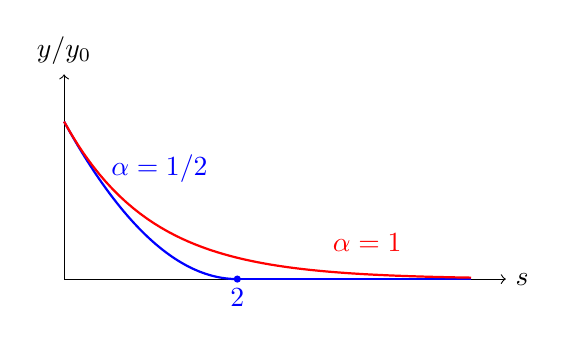
\begin{tikzpicture}[x=1.1cm,y=2cm]
\draw[->](0,0)--(5.1,0)node[right]{$s$};\draw[->](0,0)--(0,1.3)node[above]{$y/y_0$};
\draw[blue,thick,domain=0:2,samples=60]plot(\x,{(1-\x/2)^2});\draw[blue,thick](2,0)--(4.7,0);
\draw[red,thick,domain=0:4.7,samples=60]plot(\x,{exp(-\x)});
\fill[blue](2,0)circle(1.3pt)node[below]{$2$};\node[red]at(3.5,.23){$\alpha=1$};\node[blue]at(1.1,.7){$\alpha=1/2$};
\end{tikzpicture}}
图\ref{fv:c4:arrival}用 $s=ky_0^{\alpha-1}t$消去单位。$\alpha=1/2$时 $y/y_0=(1-s/2)^2$只在 $0\le s\le2$表示下降支路；此后按非负模型接到 $y=0$。若把平方式直接延长到 $s>2$，它反而增大，已经不满足原来的负导数方程。$\alpha=1$的指数曲线在任意有限 $s$仍为正。图形的触轴方式因此对应不同的到达时间，必须与方程和允许状态一起判断。




\section{从受力方程到过程关系}
\subsection{选择时间、位置或速度作为变量}
定质量的一维运动满足
\[
 m\frac{\dd v}{\dd t}=F(t,x,v),\qquad
 \frac{\dd x}{\dd t}=v.
\]
若 $F=F(x)$，在单调运动段有 $\dd v/\dd t=v\,\dd v/\dd x$，于是
\[
 \frac12m(v^2-v_0^2)=\int_{x_0}^xF(\xi)\dd\xi.
\]
左边来自 $\int_{v_0}^{v}mu\dd u=[mu^2/2]_{v_0}^{v}=m(v^2-v_0^2)/2$。这就是动能定理。若 $F=-kx$，则
\[
 \int_{x_0}^{x}(-k\xi)\dd\xi
 =\left[-\frac{k\xi^2}{2}\right]_{x_0}^{x}
 =-\left(\frac{kx^2}{2}-\frac{kx_0^2}{2}\right),
\]
故可将 $U(x)=kx^2/2$ 认作弹性势能。若 $F=-cv$，时间变量更便于直接分离。不同方法只是对同一局部方程选择了不同的变量，初值与方向约定应保持一致。

自变量的选择应与已知关系相配。若力只随位置变化，先求能量关系便能直接消去时间；若阻力只随速度变化，则 $\dd t=m\,\dd v/F(v)$ 可直接积出速度与时间。需要位置时，再用 $\dd x=v\,\dd t$。若已知 $v(x)$，还可以积分 $\dd t=\dd x/v(x)$。这些微分关系都必须在速度方向和单调运动段已经确定后使用。

特别要检查积分端点。例如 $v(x)$ 在某个位置趋零，$\dd x/v$ 可能仍可积，也可能使到达时间发散；仅从能量式看出存在零速位置，还不能判断是否在有限时间到达。反过来，若求得 $v^2<0$，应把它解释为该运动支路不能进入的区域，而不能给速度任意加一个复数值继续运动。


图\ref{c4deep:branches}用弹簧运动说明“先由能量求 $v^2$”会留下什么信息。设振幅为 $A$，能量式给出
\[
 v^2=\omega_0^2(A^2-x^2).
\]
相图的上半支表示向右运动，下半支表示向左运动；同一个位置通常对应两个相反速度。到 $x=A$ 时，速度为零，但恢复力向左，随后应沿下半支返回。能量式给出椭圆形状，原微分方程还给出沿椭圆运动的方向，二者共同决定实际过程。
\fig{c4deep:branches}{同一能量曲线包含去程和回程，不能由平方速度独自选择支路}{\begin{tikzpicture}
\draw[axis](-3,0)--(3.2,0)node[right]{$x$};\draw[axis](0,-2.1)--(0,2.2)node[above]{$v$};
\draw[blue,thick](0,0)ellipse(2.5 and 1.5);\draw[flow,blue](130:2.5 and 1.5)arc(130:65:2.5 and 1.5);
\draw[flow,red](-45:2.5 and 1.5)arc(-45:-110:2.5 and 1.5);
\node[below right]at(2.5,0){$A$};\node[above left]at(-2.5,0){$-A$};\node[above]at(1,1.7){向右};\node[below]at(-1,-1.7){向左};
\draw[force](2.5,0)--(1.55,0)node[below]{$F<0$};
\end{tikzpicture}}
在单调支路上用 $\dd t=\dd x/v$ 时，$\dd x$ 与 $v$ 同号，所得时间增量为正。若在转向以后仍使用正根，时间方向就会出错。图中的相椭圆是状态空间图，横轴、纵轴单位不同，不能把它当作质点在空间中的椭圆轨道。


\subsection{变质量系统与流入动量}
有链节不断从静止堆积部分加入运动部分时，“正在运动的部分”不是一个固定物质系统。若其质量为 $m(t)$、速度为 $v$，新进入的质量在地面参考系中的进入速度为零，则沿运动方向
\[
 F_{\rm ext}=\frac{\dd(mv)}{\dd t}=m\dot v+\dot m\,v.
\]
第二项用于把新加入的质量加速到运动速度。若进入质量本来就有速度，还应加入对应的动量流入项，不能无条件使用上述形式。

动量守恒与机械能守恒的使用条件不同。把静止链节突然带动到速度 $v$ 往往伴随非弹性过程，所以机械能可以损失；这不意味着能量守恒失效，而是必须计入内能等其他能量形式。

\fig{c4k-inflow}{短时间内将新质量纳入运动部分}{\begin{tikzpicture}
\draw[world](-2.2,-.25)rectangle(-1.4,.25);\node at(-1.8,0){$\dd m$};
\draw[flow](-2.2,.65)--(-1.35,.65)node[midway,above]{$u_{\rm in}$};
\draw[world](-.4,-.35)rectangle(.8,.35);\node at(.2,0){$m,v$};
\draw[force,red](-.3,.65)--(.75,.65)node[midway,above]{$F_{\rm ext}$};
\draw[flow](1.2,0)--(2.8,0)node[midway,above]{$\dd t$};
\draw[world](3.2,-.4)rectangle(5.7,.4);\node[align=center]at(4.45,0){$m+\dd m$\\$v+\dd v$};
\draw[flow](3.8,.65)--(5.3,.65);
\end{tikzpicture}}
图 \ref{c4k-inflow} 中，把原运动部分与即将加入的 $\dd m$ 一同作为短时物质系统。初动量是 $mv+u_{\rm in}\dd m$，末动量是 $(m+\dd m)(v+\dd v)$。将外力冲量 $F_{\rm ext}\dd t$ 加到初动量上，展开末动量并舍去二阶小量 $\dd m\,\dd v$，得到
\begin{equation}\label{eq:c4inflow}
 m\dot v=F_{\rm ext}+(u_{\rm in}-v)\dot m.
\end{equation}
式\eqref{eq:c4inflow}在 $u_{\rm in}=0$ 时才恢复前式。所有速度必须在同一个惯性参考系中取值，不能把相对进入速度直接当作地面速度代入。

对于原先静止的微小质量，它被带到速度 $v$ 所需动量为 $v\dd m$，动能却是 $v^2\dd m/2$。维持运动部分的外力还可能通过合并过程产生不可逆能量损失，因而动量方程不能替代能量方程。题目若要求外力功率，应同时追踪运动部分的质量增加和速度改变，而不只是对单个质点的 $mv^2/2$ 求导。

\section{小振动与线性化}
\subsection{恢复系数和有效惯量}
平衡点 $q_0$ 附近令 $\eta=q-q_0$。若动能与势能可写成
\[
 T=\frac12M_{\rm eff}\dot\eta^2+\text{高阶项},\qquad
 U=U_0+\frac12K_{\rm eff}\eta^2+\text{高阶项},
\]
且 $M_{\rm eff},K_{\rm eff}>0$，则保留扰动一阶项的线性化运动方程为
\[
 M_{\rm eff}\ddot\eta+K_{\rm eff}\eta=0,\qquad
 \omega_0=\sqrt{K_{\rm eff}/M_{\rm eff}}.
\]
这里两个“有效”量必须由同一广义坐标定义：对长度坐标，它们可分别具有质量、劲度系数的单位；对角坐标，有效惯量通常是转动惯量。

为了求解而不只识别方程，试取 $\eta=\e^{rt}$，则 $\dot\eta=r\e^{rt}$、$\ddot\eta=r^2\e^{rt}$，代入后得到 $r^2+\omega_0^2=0$，即 $r=\pm\mathrm i\omega_0$。由 $\e^{\mathrm i z}=\cos z+\mathrm i\sin z$，两个实独立解是 $\cos\omega_0t$、$\sin\omega_0t$，所以
\[
 \eta=C_1\cos\omega_0t+C_2\sin\omega_0t,
 \qquad
 \dot\eta=-\omega_0C_1\sin\omega_0t+\omega_0C_2\cos\omega_0t.
\]
若 $\eta(0)=\eta_0$、$\dot\eta(0)=u_0$，便有 $C_1=\eta_0$、$C_2=u_0/\omega_0$。再写成 $\eta=A\cos(\omega_0t+\phi)$，系数比较给出 $A\cos\phi=\eta_0$、$-A\sin\phi=u_0/\omega_0$，从而同时确定振幅和相位。势能需要保留二阶，恢复作用只需保留一阶；它们正好通过 $-\dd U/\dd\eta=-K_{\rm eff}\eta$ 联系起来。

从能量得到线性化方程时，可写
$\dd(T+U)/\dd t=\dot\eta(M_{\rm eff}\ddot\eta+K_{\rm eff}\eta)$。在非零速度的区间令能量变化率为零，再以连续性接到转向点，便得到简谐方程。这里有效惯量取平衡点的值；若它随坐标变化，所产生的附加项应按小量阶数判断，不能在尚未线性化时就随意视为常数。

用同一坐标定义两个系数尤其重要。若改用 $\xi=b\eta$，动能中的系数变为 $M_{\rm eff}/b^2$，势能中的系数也变为 $K_{\rm eff}/b^2$，二者之比保持不变。因此固有频率是物理系统的性质，不能随选择长度坐标还是角坐标而改变。若算出两种坐标给出不同频率，通常是惯量或恢复系数遗漏了几何因子。

\subsection{单摆的自变量与近似}
摆角 $\theta$ 是随时间变化的未知函数，时间 $t$ 是自变量。沿圆弧切向列方程得
\[
 ml\ddot\theta=-mg\sin\theta,\qquad
 \ddot\theta+\frac gl\sin\theta=0.
\]
在$|\theta|\ll1$、角度采用弧度时，$\sin\theta\simeq\theta$，线性方程为$\ddot\theta+(g/l)\theta=0$。代入简谐解的$\ddot\theta=-\omega_0^2\theta$，得到$(-\omega_0^2+g/l)\theta=0$，所以非零振动的$\omega_0=\sqrt{g/l}$。精确势能为$mgl(1-\cos\theta)$，小角近似为$mgl\theta^2/2$；动能为$ml^2\dot\theta^2/2$。摆长改变惯量与恢复系数，所以不能只比较重力的大小。

\fig{c4k-pendulum}{角坐标同时决定摆球的路径、惯量与势能}{\begin{tikzpicture}[scale=.85]
\coordinate(O)at(0,2.8);\coordinate(P)at(1.4,.375);
\draw[world](O)--(P)node[midway,right]{$l$};\draw[guide](O)--(0,0);
\draw(0,2)arc(-90:-60:.8);\node at(.3,1.75){$\theta$};
\fill(P)circle(3pt)node[right]{$m$};\draw[force](P)--++(0,-.8)node[right]{$mg$};
\draw[guide](0,.375)--(P);\draw[dim](-.55,0)--(-.55,.375);
\node[left]at(-.55,.3){$l(1-\cos\theta)$};
\node[above]at(O){$O$};
\end{tikzpicture}}
图 \ref{c4k-pendulum} 中，沿绳的约束力与切向位移垂直，切向运动只需保留重力的切向投影。选 $\theta$ 为坐标，速度大小为 $l|\dot\theta|$，所以有效惯量是 $ml^2$；势能在零点附近的二阶项为 $mgl\theta^2/2$，恢复系数是 $mgl$，二者之比才给出 $g/l$。

小角近似的对象是整段运动中允许出现的最大摆角，而不只是经过最低点时的瞬时角度。最低点处 $\theta=0$ 并不能使一个大振幅摆动变成小振幅运动。若要求较高精度，恢复力中被舍去的项从 $-\theta^3/6$ 开始，周期也会出现与振幅有关的修正；采用线性解时应同时说明这一精度范围。

\subsection{黏滞阻尼与库仑摩擦}
黏滞阻力 $-c\dot x$ 连续随速度变化，弹簧振子满足
$m\ddot x+c\dot x+kx=0$。设 $\gamma=c/(2m)$、$\omega_0=\sqrt{k/m}$，特征方程为
$r^2+2\gamma r+\omega_0^2=0$。判别式决定欠阻尼、临界阻尼或过阻尼，详见例题。机械能$E=m\dot x^2/2+kx^2/2$的导数要分别计算两项：
\begin{align*}
\dot E&=\frac m2(2\dot x\ddot x)+\frac k2(2x\dot x)\\
&=\dot x(m\ddot x+kx)=-c\dot x^2\le0.
\end{align*}
最后一步代入原来的运动方程，而没有假定机械能守恒。

干摩擦则在滑动时大小近似恒定，方向随速度反转；静止时静摩擦在允许范围内取值以维持平衡。不能把滑动摩擦的符号函数直接延伸成零速时唯一的力。判断是否再次反向，必须在每个停点重新检查静摩擦条件。

\fig{c4k-friction}{连续阻力与静摩擦的零速行为不同}{\begin{tikzpicture}
\draw[axis](-2.6,0)--(3,0)node[right]{$v$};\draw[axis](0,-1.8)--(0,2)node[above]{$F$};
\draw[blue,domain=-2:2]plot(\x,{-.75*\x});
\draw[green!50!black,line width=2pt](0,-1.3)--(0,1.3);
\draw[red,very thick](-2,.9)--(0,.9);\draw[red,very thick](0,-.9)--(2,-.9);
\node[left,red]at(-2.05,.9){$+F_k$};\node[right,red]at(2.05,-.9){$-F_k$};
\node[blue,below right]at(2,-1.5){$-cv$};
\node[green!50!black,right]at(.35,1.45){$|F|\le F_s\quad(v=0)$};
\end{tikzpicture}}
图 \ref{c4k-friction} 的蓝线在零速处连续过原点，表示黏滞阻力随速度消失；红线在速度两侧分别为定值，表示大小为 $F_k$ 的滑动摩擦；绿色线段表示最大静摩擦力为 $F_s$ 时的零速允许范围。它不是同一时刻作用着许多摩擦力，而是实际取值由其他外力与平衡要求共同决定。

对黏滞阻尼，机械能连续转化，振幅的包络随时间衰减；对干摩擦，滑动区间内可分段求解，每次停下后还要检查能否保持静止。两者都使机械能减少，却具有不同的零速边界。若不区分这一点，就会把实际已经停住的物体继续延伸成新的滑动半周。

\subsection{阻尼率与无量纲阻尼比}
对$m\ddot x+c\dot x+kx=0$，定义$\omega_0=\sqrt{k/m}$、$\gamma=c/(2m)$，则方程为$\ddot x+2\gamma\dot x+\omega_0^2x=0$。$\gamma$有时间倒数的量纲。再定义无量纲阻尼比$\zeta=\gamma/\omega_0=c/(2\sqrt{mk})$。特征方程的配方过程为
\[
r^2+2\gamma r+\omega_0^2=0
\quad\Longrightarrow\quad(r+\gamma)^2=\gamma^2-\omega_0^2.
\]
取平方根，再减去$\gamma$，得到
\[r_\pm=-\gamma\pm\sqrt{\gamma^2-\omega_0^2}
 =\omega_0(-\zeta\pm\sqrt{\zeta^2-1}).\]
欠阻尼、临界阻尼、过阻尼分别由 $0<\zeta<1$、$\zeta=1$、$\zeta>1$区分。比较的两个量必须同量纲，不能把有量纲的 $\gamma$直接与数字一比较。无阻尼 $c=0$应单独恢复简谐振动。

把时间改为 $\tau=\omega_0t$，导数变为 $\dot x=\omega_0x_\tau$、$\ddot x=\omega_0^2x_{\tau\tau}$，方程简化成 $x_{\tau\tau}+2\zeta x_\tau+x=0$。同一个 $\zeta$决定同一类归一化曲线，而 $\omega_0^{-1}$决定实际时间尺度。这种无量纲化同时检查了求导中的频率系数。



图\ref{c4deep:damped}固定相同的 $x(0)=x_0>0$、$\dot x(0)=0$，只比较阻尼比。欠阻尼曲线反复穿过平衡点，振荡包络衰减；临界阻尼曲线在这组初值下从同侧返回；过阻尼曲线的慢指数分量使长期回归更慢。图中各曲线的初始切线都水平，这是同一初速度的检查，而不是任意拼接三种形状。
\fig{c4deep:damped}{相同初位移和零初速度下，阻尼比改变回归过程}{\begin{tikzpicture}[x=.75cm,y=2cm]
\draw[axis](0,0)--(8.5,0)node[right]{$\omega_0t$};\draw[axis](0,-.5)--(0,1.25)node[above]{$x/x_0$};
\draw[blue,thick,domain=0:8,samples=150]plot(\x,{exp(-.2*\x)*(cos(.9797959*\x r)+.204124*sin(.9797959*\x r))});
\draw[red,thick,domain=0:8,samples=100]plot(\x,{(1+\x)*exp(-\x)});
\draw[green!50!black,thick,domain=0:8,samples=100]plot(\x,{1.0773503*exp(-.2679492*\x)-.0773503*exp(-3.7320508*\x)});
\node[blue]at(2.5,-.65){$\zeta=0.2$};\node[red]at(5,-.65){$\zeta=1$};\node[green!50!black]at(7.3,-.65){$\zeta=2$};\node[left]at(0,1){$1$};
\end{tikzpicture}}
改变初速度会改变曲线是否先远离或越过平衡点，因此应先确定特征根，再由初值确定系数，不能仅凭阻尼类别画出所有具体解。临界阻尼的重根对应 $(A+Bt)\e^{-\omega_0t}$，若只写一个指数就只有一个常数，通常无法同时满足两个初值。


\section{转动与追及中的微积分}
\subsection{定轴转动中的两种加速度}
绕固定轴转动的刚体有 $M_O=I_O\ddot\theta$。角加速度产生的切向加速度为 $r_\perp\ddot\theta$，转动还产生法向加速度 $r_\perp\dot\theta^2$。端点受恒定切向力矩时，只有角加速度恒定，端点的全部线加速度并不恒定。

求端点加速度时，切向项与法向项应按互相垂直的矢量合成。例如角加速度为常数$\beta$且从静止开始，先对$\dot\omega=\beta$带初值积分：
\[
\int_0^{\omega(t)}\dd\Omega=\beta\int_0^t\dd s,
\qquad\omega(t)-0=\beta[s]_0^t=\beta t.
\]
因此$a_\tau=r_\perp\beta$恒定，而$a_n=r_\perp\beta^2t^2$随时间增加。把“恒定角加速度”简写为“恒定加速度”，就会遗漏越来越明显的转向作用。


图\ref{c4deep:rotation}将同一端点的加速度分别画在早、晚两个时刻，图中切向方向均为转角增加方向。恒定角加速度 $\beta$ 给出相同大小的切向箭头；角速度变大后，法向箭头变长，合加速度的大小和方向都会改变：
\[
 |\bm a|=r_\perp\sqrt{\beta^2+\omega^4}.
\]
\fig{c4deep:rotation}{恒定的是切向项，法向项随角速度平方增加}{\begin{tikzpicture}[scale=.9]
\foreach \shift/\len/\name in {0/.45/{较早时刻},5/1.3/{较晚时刻}}{
\begin{scope}[xshift=\shift cm]
\draw[gray](0,0)circle(1.6);\draw[thick](0,0)--(1.6,0);\fill(1.6,0)circle(2pt)node[right]{$P$};\node[below]at(0,0){$O$};
\draw[force,blue](1.6,0)--(1.6,1)node[above]{$r_\perp\beta$};
\draw[force,red](1.6,0)--({1.6-\len},0)node[below]{$r_\perp\omega^2$};
\draw[force](1.6,0)--({1.6-\len},1)node[above left]{$\bm a$};\draw[guide](1.6,1)--({1.6-\len},1)--({1.6-\len},0);
\node at(.5,-2.1){\name};\end{scope}}
\end{tikzpicture}}
图中为比较分量，将两个时刻的局部径向统一画成水平；这不表示杆在两时刻方向相同。实际空间方向应随杆转动，只有分量大小可按上式直接比较。


\subsection{质心运动与能量分解}
若刚体同时平移和转动，总动能可分解为
$T=Mv_C^2/2+I_C\omega^2/2$。它来自各质点速度写成质心速度与相对速度后，一次矩交叉项为零。此关系与平行轴定理都依赖质心的定义，不能随意把任一点当成质心。

对多个质点分别写 $m_i\bm a_i=\bm F_i^{\rm ext}+\bm F_i^{\rm int}$，再相加。成对内力相消后，
\[
 \sum_i\bm F_i^{\rm ext}=M\bm a_C.
\]
这说明外力合力决定质心平动，却不能仅靠合力判断刚体是否转动。关于质心的外力矩进一步决定转动；只有力矩也为零时，刚体才可能保持不转。对于两质点，质心条件为 $m_1\bm r_1'+m_2\bm r_2'=0$，因此它们到质心的距离与质量成反比。

将每个速度写成 $\bm v_i=\bm v_C+\bm v_i'$，展开动能后，
\[
 \sum_i\frac12m_i v_i^2
 =\frac12Mv_C^2+
 \bm v_C\cdot\sum_i m_i\bm v_i'
 +\sum_i\frac12m_i v_i'^2.
\]
由于质心关系对时间求导给出 $\sum_i m_i\bm v_i'=0$，中间项严格消失。这说明质心平动能与相对运动能的分解具有直接的代数依据。


图\ref{c4deep:com}以等质量双球刚体展示速度分解。质心平动速度在两点都相同，相对转动速度则大小相同、方向相反，因此动能展开中的交叉项互相抵消。对不等质量系统，抵消的是带质量的速度和 $\sum m_i\bm v_i'$，而非单纯的速度矢量和。
\fig{c4deep:com}{各点共同的平动速度与绕质心的相对速度分开计算}{\begin{tikzpicture}
\draw[thick](0,0)--(4,0);\fill(0,0)circle(3pt)node[below]{$m_1$};\fill(4,0)circle(3pt)node[below]{$m_2$};\fill(2,0)circle(1.8pt)node[below]{$C$};
\foreach \x in {0,4}{\draw[force,blue](\x,0)--++(1.2,0)node[below right]{$\bm v_C$};}
\draw[force,red](0,0)--(0,-1.3)node[left]{$\bm v_1'$};\draw[force,red](4,0)--(4,1.3)node[right]{$\bm v_2'$};
\draw[force](0,0)--(1.2,-1.3)node[below]{$\bm v_1$};\draw[force](4,0)--(5.2,1.3)node[above]{$\bm v_2$};
\node at(2,-2.1){图示 $m_1=m_2$，逆时针转动};
\end{tikzpicture}}


\subsection{连线方向与追及速度}
追及问题需要对同一时间求相对位置的变化。记$\bm R=\bm r_A-\bm r_B$，两点距离$r=|\bm R|$。先对$r^2=\bm R\cdot\bm R$求导：
\[
2r\dot r=\dot{\bm R}\cdot\bm R+\bm R\cdot\dot{\bm R}
=2\bm R\cdot(\bm v_A-\bm v_B).
\]
相遇前$r>0$，可以除以$2r$；取从$B$指向$A$的$\bm e_r=\bm R/r$，得到
\[
\dot r=(\bm v_A-\bm v_B)\cdot\bm e_r.
\]
只有相对速度沿连线的投影改变距离，横向部分改变连线方向。对称性可大幅简化问题，但须先解释为什么运动规则保持该对称性，再把二维曲线化为径向或边长的一阶方程。

\fig{c4k-distance}{距离变化率取决于两端速度沿连线的投影之差}{\begin{tikzpicture}
\coordinate(B)at(0,0);\coordinate(A)at(4,0);
\draw[axis](-.4,0)--(5.8,0)node[right]{$\bm e_r$};
\fill(B)circle(1.7pt)node[below]{$B$};\fill(A)circle(1.7pt)node[below]{$A$};
\draw[force,blue](B)--(.8,1.4)node[above]{$\bm v_B$};
\draw[force,red](A)--(5.2,.9)node[above]{$\bm v_A$};
\draw[guide](.8,1.4)--(.8,0);\draw[guide](5.2,.9)--(5.2,0);
\draw[dim](0,-.65)--(4,-.65)node[midway,below]{$r$};
\end{tikzpicture}}
图 \ref{c4k-distance} 中，$\bm e_r$ 从 $B$ 指向 $A$。短时间内两点沿连线的位移分别为 $(\bm v_A\cdot\bm e_r)\dd t$ 与 $(\bm v_B\cdot\bm e_r)\dd t$，相减才是距离的一阶变化。即使两点速率相同，它们沿连线的投影也可能不同，所以不能只用两个速率直接相减。

若连线本身转动，沿垂直方向的相对速度满足 $r\dot\theta=(\bm v_A-\bm v_B)\cdot\bm e_\theta$。这与径向方程共同决定轨迹形状；只求相遇时间时，有时能借助对称性消去角度函数，但消去之前仍需说明它代表的方向关系。求得相遇时间后，还应检查距离在这一段内保持非负，并确实趋于零。

% thirty-c4-theory
